\documentclass[dvipdfmx,tikz]{standalone}
\usepackage{tikz,bm}
\begin{document}
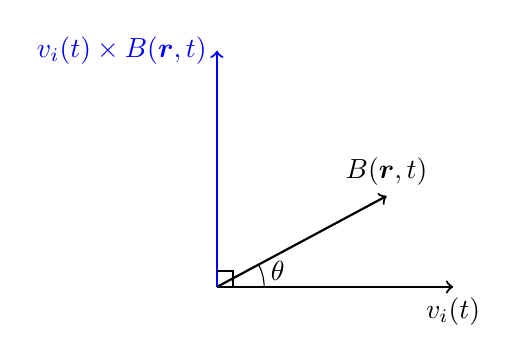
\begin{tikzpicture}
\coordinate (O)  at (0,0,0);
\coordinate (Ax) at (3,0,0);
\coordinate (Ay) at (0,3,0);
\coordinate (Az) at (0,0,-3);
\coordinate (A)  at (3,3,3);
\coordinate (AO) at (3,0,3);

% Draw axes
\draw[->,thick] (O) -- (3,0,0)
    node[anchor = north]{$v_i(t)$};
\draw[->,thick] (O) -- (1,0,-3)
    node[anchor = south]{$B(\bm{r},t)$};
\draw[->,thick,color = blue] (O) -- (0,3,0)
    node[anchor = east]{$v_i(t) \times B(\bm{r},t)$};

%
\draw (0.6,0) arc [start angle=0,end angle=29,radius=0.6] node[pos=0.7,right]{$\theta$};

% draw 
\draw[thick] (0.2,0,0) --  (0.2,0.2,0) -- (0,0.2,0);  
\end{tikzpicture}
\end{document}